%\documentclass[c,handout]{beamer}
\documentclass[c]{beamer}


\usepackage{etex}
\usetheme{Unicam}


\title{Applying Process Mining in Blockchain Transactions}

\author{Massimiliano Sampaolo}


%\usetheme{lucid}
\begin{document}

	\frame {
		\titlepage
		Supervisor: Barbara Re\\
		Second supervisor: Andrea Morichetta
    }
	
	
	\frame {
		\frametitle{Objective and Motivations}
		The thesis want to understand and define bindings between \textbf{blockchain} transactions 
		using \textbf{process mining}.\\ \vspace{20px}
		Why?
		\begin{itemize}
			\item Blockchain and process mining are hot topics in industry and academia
			\item Infer and analyse the behaviour of systems to increase their quality
			\item Give a graphical representation of processes defined by software systems
		\end{itemize}
	}
	
    
	\frame{
		\frametitle{Blockchain}

		Chain of blocks:
		\begin{figure}[H]
			\centering
			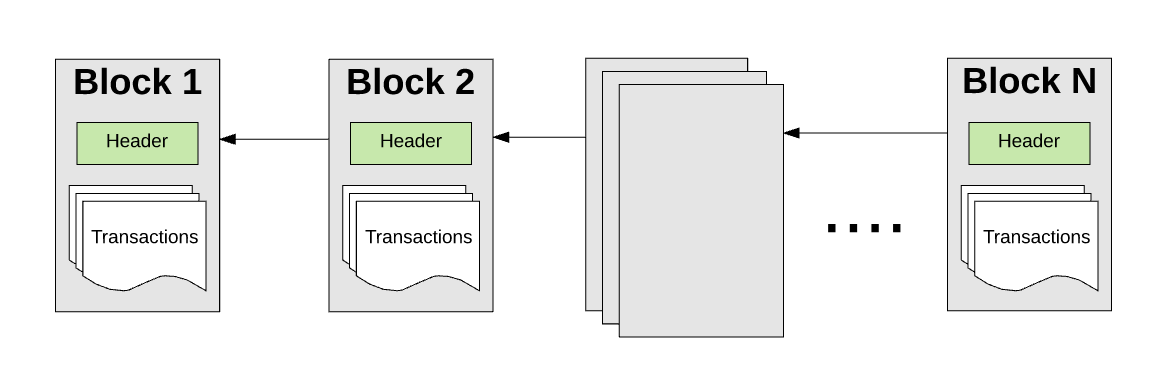
\includegraphics[width=70mm]{images/chain_of_blocks.png}
		\end{figure}

		Blockchain characteristics:
		\begin{itemize}
			\item Decentralization
			\item Trasparency
			\item Security
			\item Immutability
		\end{itemize}
		\textbf{Ethereum}: EVM, Smart Contracts and DAPP
    }
	
	
	\frame{
	    \frametitle{Business Process Management}
		
		A \textbf{Business Process} is a collection of related and structured activities undertaken by one or more 
		organisations in order to pursue some particular goal.

		\vspace{16px}
		
		\textbf{Business Process Management} (BPM) is the set of activities needed to define, optimize and monitor 
		business processes in order to make effective company’s business.

		\vspace{16px}

		\textbf{BPMN} (Business Process Model and Notation) is a standard language to grapichally represent 
		process models.
	}
	

	\frame{
		\frametitle{Process Mining}
		The idea is to discover, monitor and improve real processes by extracting knowledge from event logs readily 
		available in today's information systems.

		\vspace{16px}

		Three form of process mining:
		\begin{itemize}
			\item Process discovery
			\item Conformance checking
			\item Enhancement
		\end{itemize}

		\vspace{16px}

		Used discovery algorithms: \textbf{Heuristic Miner}, \textbf{Inductive Miner}, \textbf{Split Miner}
	}

	\frame{
		\frametitle{Heuristic Miner}
		It mines the control-flow perspective of a process model. It extends alpha algorithm by considering the frequency of traces 
		in the log. 

		\vspace{16px}

		It consists in a set of steps: 
		\begin{itemize}
			\item the identification of all the activities
			\item find the connection between activities and their frequencies
			\item dependency relation matrix is calculated
			\item final net is built from the matrix previously created
		\end{itemize}
	}

	\frame{
		\frametitle{Inductive Miner}

		It uses a divide-et-conquer approach: 

		\begin{itemize}
			\item builds a directly follow graph (DFG)
			\item filters infrequent directly-follows dependencies
			\item find the dominant operator and apply relative cut
			\item a process tree is generated from each portion
		\end{itemize}

		\vspace{16px}

		The third step is applied recursively until no more cuts are found.
	}

	\frame{
		\frametitle{Split Miner}
		
		Split Miner produces a BPMN model in five steps:

		\begin{figure}[H]
			\centering
			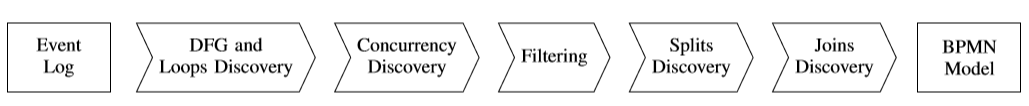
\includegraphics[width=120mm]{images/split_miner_steps.png}
		\end{figure}
	}

	\frame{
		\frametitle{Process mining tools}
		
		Different software tools are available to support process mining techniques.
		
		\vspace{16px}

		The more used are: 
		\begin{itemize}
			\item ProM
			\item Apromore
			\item Disco
		\end{itemize}
	}


	\frame{
		\frametitle{Case Studies}
		
		The methodology used for the case studies consists of several steps:
		
		\vspace{16px}

		\begin{itemize}
			\item Retrieving of transaction list from Ethereum
			\item Generation of log file starting from the transaction list
			\item Analysis of the log with discovery algoritms previously introduced
			\item Quality check of the results obtained
		\end{itemize}
	}


	\frame{
		\frametitle{RoToHive}

		\begin{figure}[t]
			\centering
			
\includegraphics[width=60mm]{images/rotohive.png}
		\end{figure}

		RotoHive is a new type of fantasy sports site that runs weekly tournaments.

		\vspace{16px}
		
		Results obtained:
		
		\begin{center}
			\label{tables:roto}
			\begin{tabular}{ | l | c | c | c |}
				\hline
				\textbf{Algorithm} & \textbf{Fitness} & \textbf{Precision} & \textbf{Generalization} \\ 
				\hline
				Split Miner & 1 & 0.20453 & 0.99892 \\ 
				\hline
				Inductive Miner & 0.99995 & 0.60294 & 0.99496 \\
				\hline
				Heuristic Miner & 0.99940 & 0.49889 & 0.99889 \\
				\hline
			\end{tabular}
		\end{center}
	}


	\frame{
		\frametitle{Lessons learned}

		Sound models discovered and pretty good quality parameters measured.

		\vspace{16px}

		The three algorithms obtained similiar results. How well an algorithm fits a specific application domain depends from 
		the domain itself regardless the fact that it uses the Blockchain.

		\vspace{16px}

		The analysis infer the logic of the system. Can be used to increase solution quality, or understand how users interact with 
		a product.
	}


	\frame{
		\frametitle{Design and implementation}
		
		The system designed recreates the methodology used in the case studies analysis.

		\vspace{16px}

		The architecture of the Mining Framework: 

		\begin{figure}[t]
			\centering
			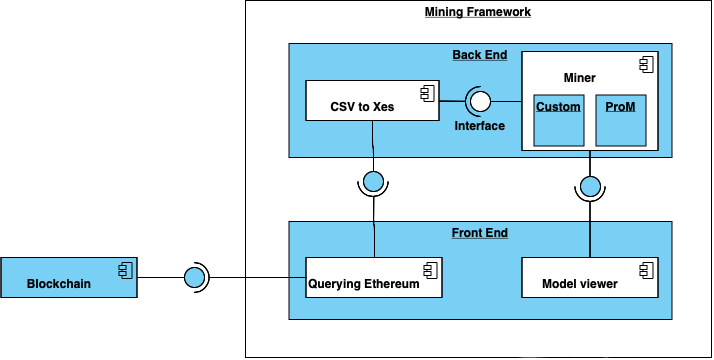
\includegraphics[width=80mm]{images/component_diagram.png}
		\end{figure}
	}
    
\end{document}